\section{Theorie}\label{sec:theorie}
Nachdem zunächst auf die verschiedenen Wechselwirkungen von elektromagnetischer Strahlung mit Materie eingegangen wird, folgt mit diesem Wissen eine Einführung in die Funktionsweise des verwendeten Germaniumdetektors.
\subsection{Wechselwirkungsprozesse von Photonen mit Materie}
Im Wesentlichen spielen drei Effekte eine wesentliche Rolle bei dem Einfall von im Versuch erzeugten Gammaquanten in Materie, wie in \autoref{fig:extinkt} dargestellt ist.
Allgemein kann die Intensität $I$ von Strahlung innerhalb eines Materials abhängig von der Eindringtiefe $x$ mithilfe der Funktion
\begin{align}
  I(x) = I_0\cdot\exp{(-\mu x)}
\end{align}
modelliert werden, wobei $\mu$ Extinktionskoeffizient oder Absorptionskoeffizient genannt wird. Dieser von verschiedenen Materialeigenschaften sowie Strahlungsenergie abhängige Paramater beschreibt, wie stark ein Material die respektive Strahlung abschwächt.
Im Anschließenden wird der zustandekommende Graph erklärt.
\begin{figure}[H]
  \centering
  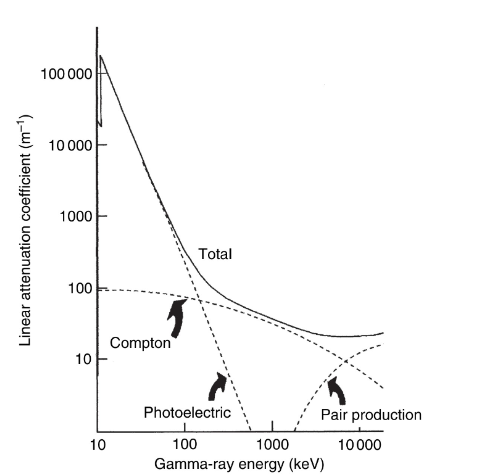
\includegraphics[scale=0.65]{Ressourcen/extinkt.png}
  \caption{Schematischer Verlauf des Extinktionskoeffizienten in Abhängigkeit der Photonenenergie\cite{gilmore}.}
  \label{fig:extinkt}
\end{figure}
\subsubsection{Photoelektrischer Effekt}
Der Photoeffekt beschreibt den Prozess, bei dem ein Gammaquant seine gesamte Energie an ein Hüllelektron eines Atoms abgibt, es herauslöst und das Atom somit ionisiert. Damit es zu diesem Verhalten kommen kann, müssen die Photonen bestimmte Energien, welche mit den Bindungsenergien der Elektronen im Atom übereinstimmen, besitzen.
Der Wirkungsquerschnitt $\sigma$, ein Maß für die Wahrscheinlichkeit eines Wechselwirkungsprozesses, sinkt für den Photoelektrischen Effekt mit steigender Energie, was sich in \autoref{fig:extinkt} in einer Abnahme des Extinktionskoeffizienten $\mu$ widerspiegelt.
Konkret ergibt sich als quantitative Abhängigkeit 
\begin{align}
  \sigma \sim Z^\alpha E^\delta\text{,}
\end{align}
wobei $Z$ die Kernladungszahl des Absorbers, $E$ die Strahlungsenergie und $\alpha \in(4,5)$ und $\delta = -3,5$ die Exponenten der Proportionalität beschreiben.
Ebenso ist ersichtlich, dass dieser Prozess für Photonenenergien bis zu $\SI{100}{\kilo\electronvolt}$ dominiert.

\subsubsection{Compton-Effekt}
Ebenso können Photonen an Hüllenelektronen im Korpuskelmodell des Lichts unelastisch gestreut werden und so ein Energieübertrag geleistet werden, wodurch sich die Wellenlänge des Photons verlängert. Im Gegensatz zum Photoeffekt wird bei diesem Prozess nur ein Teil der Energie übertragen und das Photon kann den Absorber wieder verlassen.
Als Abhängigkeit der Energie des gestreuten Photons $E_\gamma'$ von der Energie des einfallenden Photons $E_\gamma$ und dem Streuwinkel $\theta$, mit Annahme eines ruhenden Elektrons ergibt sich
\begin{align}
  E_\gamma' = \frac{E_\gamma}{1+\frac{E_\gamma}{m_0c^2}(1-\cos{\theta})}\text{,}\label{eqn:compton}
\end{align}
wobei $m_0$ die Ruhemasse des Elektrons und $c$ die Lichtgeschwindigkeit beschreibt.
Aus \autoref{eqn:compton} ist ersichtlich, dass der maximale Energieübertrag von Photon auf Elektron
\begin{align}
  E_{\text{max}} = E_\gamma\left(1-\frac{1}{1+\frac{2E_\gamma}{m_0c^2}}\right)\label{eqn:Comptonmax}
\end{align}
bei einem Streuwinkel von $\SI{180}{\degree}$ stattfindet.
Ausgehend von dem Winkungsquerschnitt 
\begin{align}
  \sigma_\text{Compton}=\frac{3}{4} \sigma_\text{Thomson} = \frac{3}{4}\cdot\frac{8\pi}{3}r_e^2\text{,}
\end{align}
wobei $r_e= \frac{e_0}{4\pi\epsilon_0c^2m_0}$ den klassischen Elektronenradius beschreibt, ergibt sich nach Ableitung nach der Energie des gestreuten Photons der differentielle Wirkungsquerschnitt
\begin{align}
  \frac{d \sigma}{d E} = \frac{\pi r_{\text{e}}}{\epsilon E_\gamma} \left(2 - \frac{2 E}{\epsilon \left(E_\gamma - E \right)}+ \frac{E^2}{\epsilon^2 \left(E_\gamma - E \right)^2} + \frac{E^2}{E_\gamma \left(E_\gamma - E \right)}\right).
  \label{eqn:Wirkungsquerschnitt}
\end{align}
Des weiteren ergibt sich ausgehend von der Klein-Nishina-Formel die Abhängigkeit
\begin{align}
  \frac{d \sigma}{d \Omega}=\frac{r_e^2}{2\left[1+\epsilon\left(1-\cos \theta_\gamma\right)\right]^2}\left(1+\cos ^2 \theta_\gamma+\frac{\epsilon^2\left(1-\cos \theta_\gamma\right)^2}{1+\epsilon\left(1-\cos \theta_\gamma\right)}\right).
\end{align}
für den differentiellen Wirkungsquerschnitt nach Raumwinkel $d\Omega$, wobei die Abkürzung 
\begin{align*}
  \epsilon=\frac{E_\gamma}{m_0c^2} 
\end{align*}
verwendet wurde.
Wird der Wirkungsquerschnitt pro Atom unter der Annahme von freien Elektronen betrachtet, gilt die Abhängigkeit
\begin{align}
  \sigma_\text{Compton}^\text{Atom}=Z\cdot \sigma_\text{Compton}\text{.}
\end{align}
\subsubsection{Paarerzeugung}
Die letzte hier erwähnte Wechselwirkung ist die Paarerzeugung, bei welcher ein Photon im Coulomb Feld des Atomkerns in ein Elektron-Positron Paar umgewandelt wird.
Somit muss, um Paarerzeugung zu ermöglichen, für die Energie des Photons
\begin{align}
  E_\gamma \approx 2m_ec^2
\end{align}
gelten. Gemäß \autoref{fig:extinkt} dominiert dieser Prozess für Gamma-Quant-Energien größer als $\SI{1}{\mega\eV}$.
\subsection{Funktionsweise des Germaniumdetektors}
Halbleiterdetektoren, wie der im Versuch verwendete Germanium-Detektor, sind wichtige Instrumente zur Detektion und Analyse von Gammastrahlung. Ihre Funktion basiert auf den physikalischen Eigenschaften von Halbleitermaterialien und der oben beschriebenen Wechselwirkung der Gammastrahlung mit Materie. Im Folgenden wird die Funktionsweise eines Halbleiterdetektors beschrieben.

\subsubsection{Grundlagen}
Ein Halbleiterdetektor besteht im wesentlichen aus einer Halbleiterdiode, die aus zwei benachbarten Zonen besteht: einer \textit{n-dotierten} und einer \textit{p-dotierten} Zone, in welcher Atome mit relativ höherer oder niedrigerer Elektronenzahl ins Material eingebracht sind. An der Grenzfläche zwischen diesen beiden Zonen bildet sich eine sogenannte Verarmungszone, in der fast keine freien Ladungsträger vorhanden sind.

\subsubsection{Wechselwirkung von Strahlung mit dem Detektor}
Trifft Gammastrahlung auf die Verarmungszone des Halbleiters und hat die Energie der Strahlung einen Wert oberhalb der Bandlücke des Materials, so können die Photonen Elektronen aus dem Valenzband in das Leitungsband anregen. Dies führt zur Bildung von Elektron-Loch-Paaren im Detektor. Die Anzahl dieser Paare ist proportional zur absorbierten Energie der Gammastrahlung:
\begin{align}
  n = \frac{E_{\text{abs}}}{\epsilon_\text{Paar}},
\end{align}
wobei $E_{\text{abs}}$ die Energie der absorbierten Strahlung und $\epsilon_\text{Paar}$ die Energie ist, die benötigt wird, um ein Elektron-Loch-Paar zu erzeugen.

\subsubsection{Signalverarbeitung}
Die Elektronen bewegen sich aufgrund ihrer negativen Ladung zur $n$-Schicht, während die Löcher in Richtung der $p$-Schicht wandern. Auf dem Weg wechselwirken die Elektronen aufgrund ihrer hohen Energie weiter mit dem Detektor und erzeugen Sekundäre Elektron-Loch Paare. Dieser letzliche Ladungstransport erzeugt einen Strompuls, der mit einem angeschlossenen Strommesser detektiert werden kann. Die Höhe des Strompulses ist direkt proportional zur Energie der deponierten Gammastrahlung.
\subsection{Spektrum eines monochromatischen Gamma-Strahlers}
Wie in \autoref{fig:cs137} beispielhaft für Cs-137 zu sehen, weist das Spektrum einer Gammaquelle mehrere charakteristische Stellen auf.
\begin{figure}[H]
  \centering
  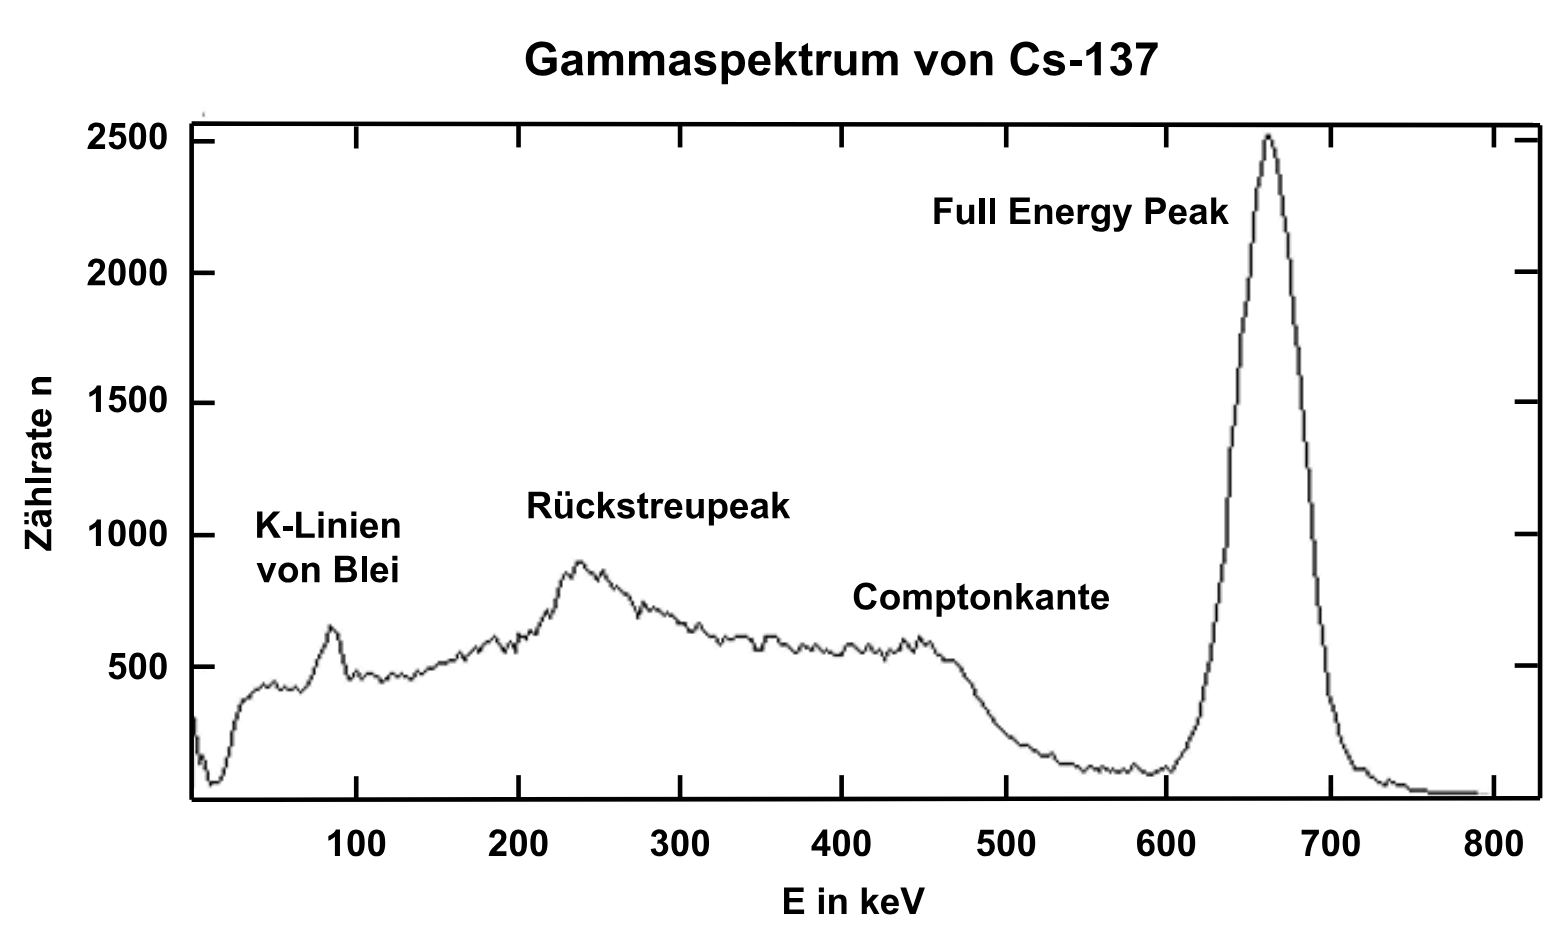
\includegraphics[scale=0.3]{Ressourcen/cs137.png}
  \caption{Spektrum einer Caesium-137 Quelle.\cite{leifics137}.}
  \label{fig:cs137}
\end{figure}
Wie oben erwähnt ist die Energiedeponierung durch Compton-Streuung nicht diskret, wodurch das im Spektrum sichbare Compton-Kontinuum entsteht. Dieses Erstreckt sich von $E_\text{min}$, festgelegt durch das verwendete Material des Halbleiterdetektors, bis zur Compton-Kante
\begin{align} 
  E_\text{max}=\frac{E_\gamma\cdot2\epsilon}{1+2\epsilon}\text{,}
\end{align}
wie aus \autoref{eqn:Comptonmax} hervorgeht. Im Versuchsfall liegt liegt $E_\text{min}$ bei etwa $\SI{40}{\kilo\eV}$.
Des weiteren ist der Rückstreupeak ein charakteristischer Bereich im Gammaspektrum, der durch Photonen entsteht, die außerhalb des Detektors durch den Compton-Effekt gestreut wurden und anschließend mit reduzierter Energie in den Detektor zurückkehren. Die Energie dieser Photonen kann durch die Formel
\begin{align} 
E_{\text{Rück}} = \frac{E_\gamma}{1 + \frac{2E_\gamma}{m_e c^2}}
\end{align}
berechnet werden. Der Rückstreupeak erscheint im Spektrum unterhalb der Compton-Kante.
Der in \autoref{fig:cs137} prominenteste Full Energy Peak/ Photopeak steht für den Fall der restlosen Energiedeponierung des Gammaquants durch den Photoeffekt, optional nach vorheriger Compton-Streuung. Der Peak repräsentiert somit direkt die Energie der einfallenden Gammaquanten. 